\subsection{Proposed Solution}

wada wada

\subsubsection{Formal specification}
The formalisation and extension of the WAC specification will be
attained through subsequent refinement phases. In the tradition of
functorial semantics\cite{lawvere1963functorial, bonchi2017functorial},
a preliminary algebraic model will provide a concise, consistent and
unambiguous interpretation of WAC in terms of basic structures and
structure-preserving transformations in the elementary theory of the
categories of sets\cite{lawvere1964elementary, leinster2014rethinking}.
We will then engage with the WAC authors on GitHub to validate and
refine the model. Following that, we will devise a specification extension
to make the evaluation model more flexible so as to allow the evaluation
of access control policies expressed in terms of predicates on a generic
set---i.e., functions from a set $X$ to the Boolean algebra $\{0,1\}$.
At the same time, we will investigate another specification extension
to accommodate data sharing through functional and homomorphic encryption
techniques. Finally, we will encode the formal specification in an
advanced programming language (either Haskell\cite{peytonjones:h98}
or Idris\cite{brady2013idris}) which we will then leverage to produce
a machine-checked proof of correctness of the resulting computer program.
The resulting (correct!) executable specification will be submitted to
the Solid project for consideration as a future version of WAC.

To illustrate our approach, consider WAC's authorisation process (\S 5)
and ACL resource discovery (\S 3.1). One possible interpretation of
the specification is that a server arranges information resources
in a tree $ResTree$ and, likewise, maintains an ACL resource tree
$ACLResTree$ containing the policies that protect the resources in
$ResTree$. Neither tree is empty. Now a tree is the same as a poset
with a terminal object. Each child-parent edge is a morphism
$\ftype{child}{parent}$ and the tree's root node is then terminal.

\begin{wrapfigure}{r}{0.5\textwidth}
  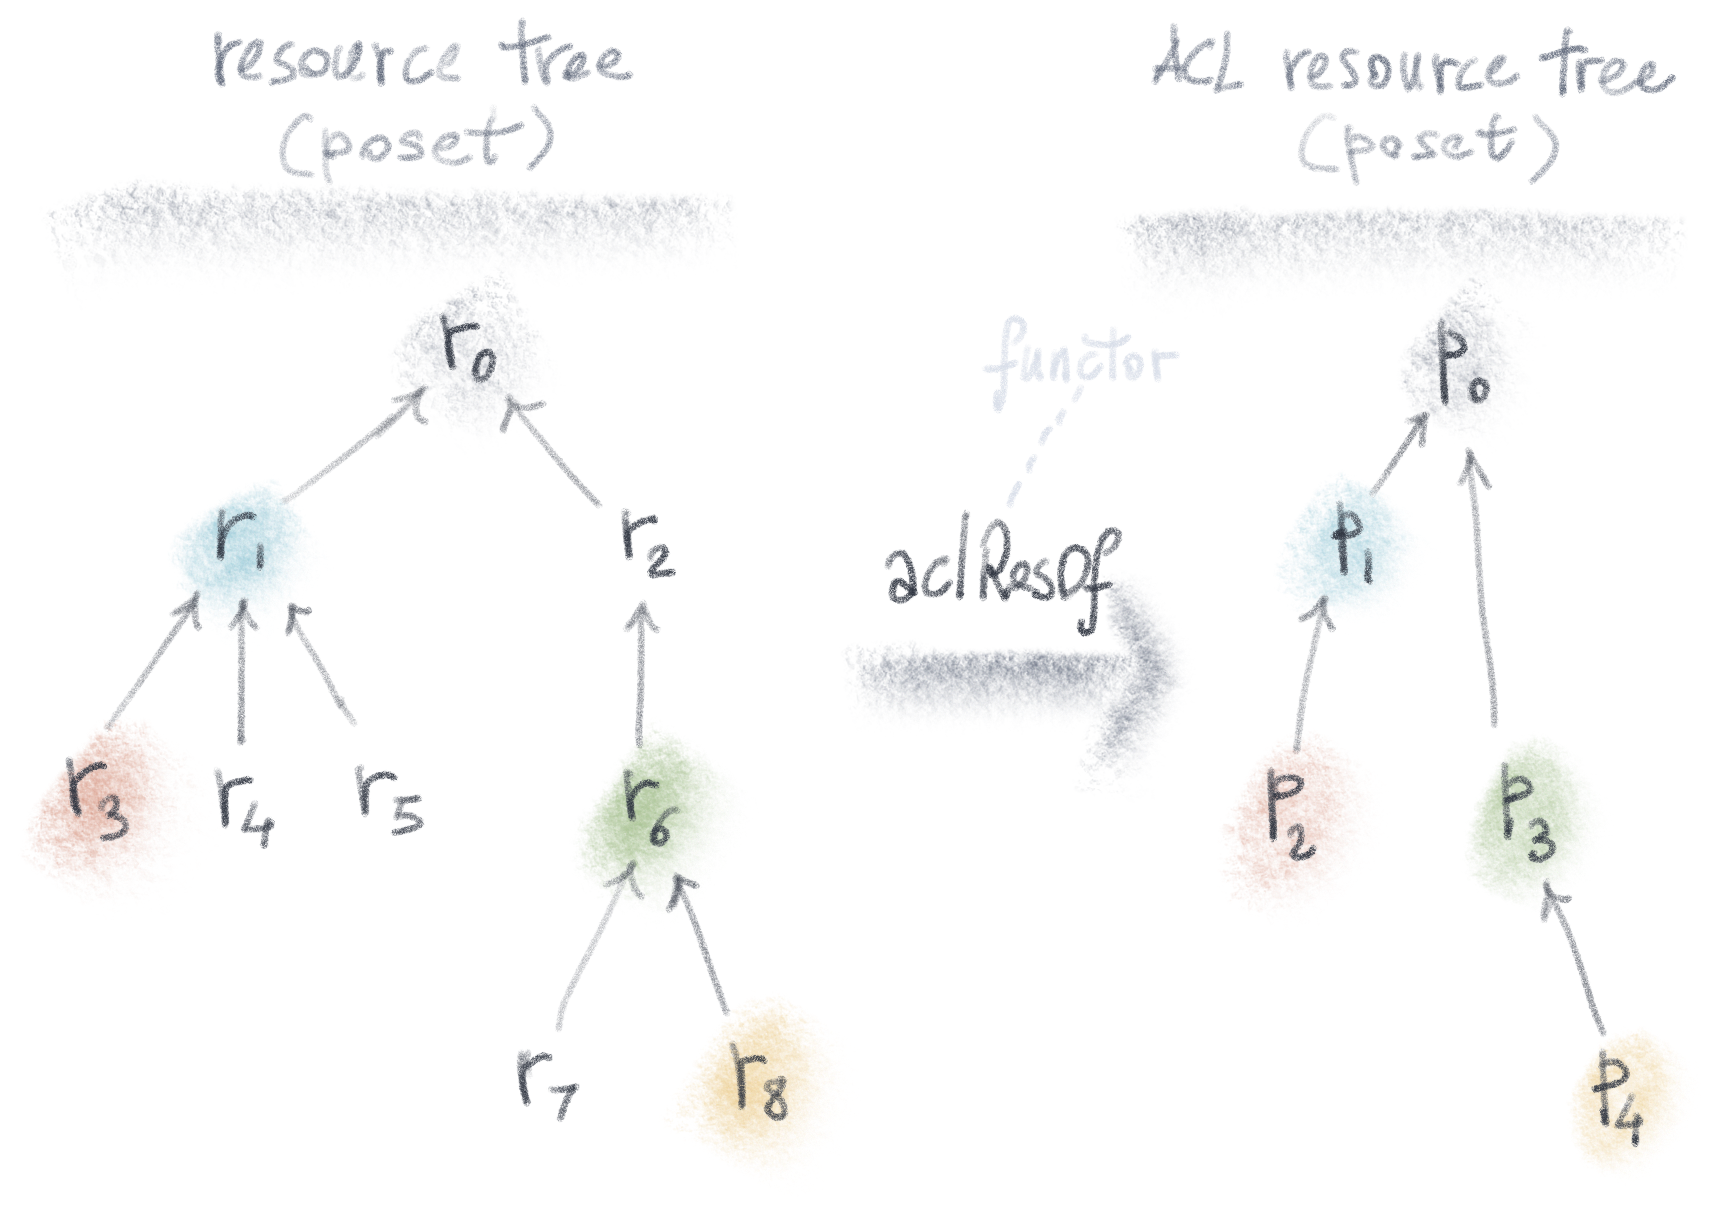
\includegraphics[width=0.5\textwidth]{effective-acl}
  % \caption{$aclResOf$ functor.}
  % \label{fig:aclResOf}
\end{wrapfigure}

On receiving an HTTP request, the server determines the ACL resource
that protects the resource which the request targets. We model this
lookup procedure as a functor $\fsig{aclResOf}{ResTree}{ACLResTree}$.
Thus, each path $t_0 \rightarrow t_1 \rightarrow \ldots \rightarrow t_m$ in $ResTree$
goes to a path $u_0 \rightarrow u_1 \rightarrow \ldots \rightarrow u_n$
in $ACLResTree$ with $n \leq m$. Then if $r$ is the resource that
the incoming HTTP request targets, $aclResOf(r)$ is its corresponding
ACL resource. The figure on the right depicts an example $aclResOf$
functor. Colours hint how the functor maps resource nodes to ACL
resource nodes: $r_0$, $r_1$, $r_3$, $r_6$ and $r_8$ are mapped,
respectively, to $p_0$, $p_1$, $p_2$, $p_3$ and $p_4$. Since paths
must go to paths, $r_4$ and $r_5$ are forced to map to $p_1$. Ditto
for $r_7$ that must go to $p_3$. Finally, $r_2$ could either map to
$p_0$ or $p_3$, but in our example $aclResOf(r_2) = p_0$.

To translate an arbitrary $aclResOf$ functor into e.g. Haskell code,
observe that such a functor can be defined in terms of the function
$path$ which finds the path from the root of the tree to a node satisfying
a given predicate $p$. In turn, $path$ can easily be defined on a
canonical multi-way tree structure with the help of the standard
list processing function $concatMap$. It is just as easy to prove
$path$ correct by induction. Below is the corresponding Haskell code.
\begin{lstlisting}[language=Haskell]
  data Tree a = Node a [Tree a]

  path :: (a -> Bool) -> Tree a -> [a]
  path p = collect []
    where
    collect xs (Node a ts) | p a       = a:xs
                           | otherwise = concatMap (collect (a:xs)) ts
\end{lstlisting}

In conclusion, we have turned an informal, ambiguous specification
into a precise model that can be reasoned about mathematically and
have encoded it into a program which can be proved to satisfy the
specification. Crucially, functoriality captures WAC's idea of ACL
resource inheritance. For example, with reference to the figure above,
$r_7$ "inherits" $r_6$'s ACL resource, $p_3$, because the functor
preserves paths, hence, necessarily, $aclResOf(r_7) = p_3$. Thus,
the lengthily WAC discussion about effective ACL resources and ACL
resource discovery can be distilled into the concise statement that
there is a given functor  $\fsig{aclResOf}{ResTree}{ACLResTree}$.


\subsubsection{Access control policies}
As mentioned earlier, access control policies can be expressed in
terms of predicates. In fact, the Boolean algebra operations on
$\mathbb{B} = \{0,1\}$ are readily lifted to any function space
$\mathbb{B}^X$ by point-wise definition---e.g., for any $p,q \in \mathbb{B}^X$
define $p \wedge q$ as $(p \wedge q)(x) = p(x) \wedge q(x)$. We will
exploit this fact to design a domain-specific language embedded in
Idris or Haskell (EDSL\cite{gibbons2014folding}) which allows policy
authors to express access control rules in a language close to plain
English. For example, to state that an administrator can read or write
a Web resource whereas anyone named Joe and born after 1995 is allowed
to perform any operation on that resource, the policy author would
write something similar to the following
\begin{lstlisting}
  role admin can read or can write
  or anyone who has name (== "joe"), has dob (> 1995) can do anything
\end{lstlisting}
The policy interpreter parses the above into predicates on a given
set $X$ (typically the data contained in a Web request, which, in
this case, the policy author expects to have $name$ and $dob$ fields)
and operations on $\mathbb{B}^X$, then uses these operations to combine
and evaluate the predicates. Note that the policy interpreter is
embedded, thus the user benefits from the read-eval-print loop
(REPL) of the host language for developing and testing policies
interactively.

The policy-as-a-predicate WAC extension mentioned in the previous
section will enable seamless integration of our EDSL in the Solid
ecosystem. End-users will be able to express access control policies
in a more concise, direct and natural way than it is currently possible
with ODRL or Access Control Policy---the go-to RDF ontologies for
ACL policies in Solid. For comparison purposes, expressing the same
example EDSL policy as earlier in ODRL would require a page of terse
Turtle as it can be evinced from the following snippet which only
encodes the small fragment $dob (> 1995)$
\begin{lstlisting}
  @base <http://example.com/> .
  @prefix ex: <http://example.com/> .
  @prefix odrl: <http://www.w3.org/ns/odrl/2/> .
  @prefix xsd: <http://www.w3.org/2001/XMLSchema#> .

  ex:dob a odrl:Constraint ;
      odrl:leftOperand odrl:dateTime ;
      odrl:operator odrl:lt ;
      odrl:rightOperand "1995"^^xsd:date .
\end{lstlisting}
